\section{Evaluation}
\label{sec:evaluation}

We evaluate \sys on both axes of dual efficiency: training
efficiency and agent-task efficiency. We validate training
correctness against \megatron on both pretraining loss curves and
downstream accuracy in
Appendix~\ref{sec:appendix:model-quality}.
This section is organized to answer the following questions:
\squishlist
  \vspace{-2pt}
  \item Does \sys deliver competitive training throughput against production frameworks?~(\S\ref{sec:eval:training})
  \vspace{-2pt}
  \item Does \sys offer higher agent-task efficiency than production frameworks?~(\S\ref{sec:eval:agent})
  \vspace{-2pt}
  \item How much do agent skills improve agent-task efficiency on \sys?~(\S\ref{sec:eval:skills-ablation})
  \vspace{-2pt}
  \item Where do the per-framework differences in agent cost come from
  on a single concrete task?~(\S\ref{sec:eval:case})
  \vspace{-2pt}
\squishend

\subsection{Training Efficiency}
\label{sec:eval:training}







\begin{table}[t]
  \centering
  \small
  \caption{Training throughput across frameworks.
  We report the aggregate tokens per second as the training throughput.
  ``---'' denotes not supported; ``OOM'' denotes out of memory.
  }
  \label{tab:training-throughput}
  \setlength{\tabcolsep}{3pt}
  \begin{tabular}{lll|ccc}
    \toprule
    Model & Hardware & Parallelism / SeqLen / Precision & \megatron & \torchtitan & \sys \\
    \midrule
    GPT-OSS-20B      & 1$\times$8-B200 & PP2,DP1,CP1,EP4 / 8192 / BF16 & 129.5K & ---\protect\footnotemark{} & 140.9K \\
    Qwen3-30B-A3B    & 1$\times$8-B200 & PP2,DP1,CP1,EP4 / 8192 / FP8  & 106.2K & OOM & 134.5K \\
    Qwen3-30B-A3B    & 2$\times$8-H100 & PP2,DP1,CP1,EP8 / 2048 / BF16 & 126.7K & 90.5K  & 124.9K \\
    Qwen3-30B-A3B    & 4$\times$8-H100 & PP4,DP1,CP1,EP8 / 4096 / BF16 & 264.1K & OOM & 280.0K \\
    DeepSeek-V2-Lite & 1$\times$8-H100 & PP2,DP1,CP1,EP4 / 2048 / BF16 & 107.3K & 74.1K  & 114.6K \\
    \bottomrule
  \end{tabular}
\end{table}
\footnotetext{\torchtitan does support GPT-OSS-20B training, but not with pipeline parallelism.}

We compare \sys~(\texttt{23db182}), \megatron~\cite{narayanan2021efficientlargescalelanguagemodel}~(\texttt{3bec9aa})
and \torchtitan~\cite{liang2025torchtitanonestoppytorchnative}~(\texttt{d84e83d}) on three
representative MoE models (GPT-OSS-20B~\cite{openai2025gptoss120bgptoss20bmodel},
Qwen3-30B-A3B~\cite{yang2025qwen3technicalreport}, and
DeepSeek-V2-Lite~\cite{deepseekai2024deepseekv2strongeconomicalefficient})
under matched parallelism (PP, DP, CP, EP), sequence length, and precision.
Configurations span single-node and multi-node deployments on
NVIDIA H100 and B200 GPUs.
For \megatron, we follow NVIDIA's documented best practices\protect\footnote{\url{https://docs.nvidia.com/nemo/megatron-bridge/nightly/training/moe-optimization.html}}.
\deepspeed is excluded as it does not currently support PP combined with EP for MoE
training\protect\footnote{Verified at commit \texttt{44c51e3}: the
Megatron-DeepSpeed integration script states ``Currently we don't
support PP for MoE.''}, so it cannot run any of the configurations in
our suite.

To ensure the MoE router exhibits steady-state load-balanced
routing across frameworks and thus comparable throughput,
we load public model checkpoints rather than random initializations.
Each experiment runs 25 steps, and we report the median step
time over the last 10. We omit Model FLOPs Utilization
(MFU)~\cite{chowdhery2023palm} because Tensor Core peak FLOPS differs
between BF16 and FP8, making the metric ambiguous for 
mixed-precision steps.
Training hyperparameters follow
Appendix~\ref{sec:appendix:model-quality}.

As \autoref{tab:training-throughput} shows, \sys matches or exceeds
\megatron on 4 of 5 configurations, and stays within 1.4\% of
\megatron on the fifth. This parity comes from optimizations such
as DualPipeV's compute--communication overlap and
\texttt{torch.compile(fullgraph=True)}. These results demonstrate
that a compact, Python-native codebase can achieve competitive
training throughput.

\subsection{Agent-Task Efficiency}
\label{sec:eval:agent}

In this section, we evaluate agent-task efficiency across
frameworks.
We run \sysbench (\S\ref{sec:benchmark}) on \megatron, \torchtitan,
and \sys with Claude Code (Opus~4.7 at
\texttt{xhigh} effort\protect\footnote{\url{https://platform.claude.com/docs/en/build-with-claude/effort}})
as the fixed agent. Each task runs three times and we report
medians; hardware configuration, task descriptions, correctness criteria, and per-attempt
values are described in Appendix~\ref{sec:appendix:tasks} and
\ref{sec:appendix:per-task-results}. Opus~4.7 completed
every task across all attempts and frameworks with no failure.

\MyPara{Q\&A.}
Answering a question requires locating where a behavior lives in
the codebase. We omit Session Duration (all tasks finish in under
three minutes) and Active GPU Time (no training runs). All 12
questions are answered correctly across attempts and frameworks
(grading details in
Appendix~\ref{sec:appendix:tasks:qa-correctness}).
Across the 12 questions, the agent uses up to 67\% fewer Agent Turns to reach the final answer on \sys than on \megatron.
A compact codebase and the
absence of implicit indirection shrink the search space, lowering
Per-Turn Context (\autoref{tab:agent-efforts-codebaseqa})
accordingly.

\begin{table}[t]
  \centering
  \small
  \vspace{-7pt}
  \caption{Per-question agent effort on the Q\&A task suite
  (\S\ref{sec:benchmark}); Q1--Q12 are described in
  Appendix~\ref{sec:appendix-codebaseqa}. Each metric reports the
  median of three independent attempts. Lower is more efficient.
  Headers abbreviate \megatron, \torchtitan, and \sys.}
  \label{tab:agent-efforts-codebaseqa}
  \begin{tabular}{c|rrr|rrr|rrr}
    \toprule
       & \multicolumn{3}{c|}{Agent Turns}    & \multicolumn{3}{c|}{Per-Turn Context}            & \multicolumn{3}{c}{Output Tokens} \\
    \# & Megatron & Titan & Pith & Megatron & Titan & Pith & Megatron & Titan & Pith \\
    \midrule
    Q1  & 33         & 18          & \textbf{15} & 45.8K          & 44.3K          & \textbf{33.4K} & 9.0K           & 7.1K           & \textbf{4.1K}  \\
    Q2  & 54         & 28          & \textbf{18} & 41.2K          & 43.5K          & \textbf{35.9K} & 10.7K          & 7.8K           & \textbf{5.4K}  \\
    Q3  & 14         & 14          & \textbf{13} & \textbf{31.3K} & 36.1K          & 34.1K          & \textbf{3.4K}  & 3.5K           & 3.4K           \\
    Q4  & 36         & 26          & \textbf{16} & 41.3K          & 39.7K          & \textbf{31.1K} & 10.0K          & 6.9K           & \textbf{5.2K}  \\
    Q5  & 48         & \textbf{19} & 21          & 46.5K          & 41.7K          & \textbf{33.8K} & 10.7K          & 4.8K           & \textbf{4.6K}  \\
    Q6  & 12         & \textbf{4}  & 11          & 36.4K          & 29.9K          & \textbf{27.9K} & 4.5K           & \textbf{2.3K}  & 3.3K           \\
    Q7  & \textbf{9} & 12          & 14          & 31.5K          & \textbf{30.0K} & 31.5K          & \textbf{2.6K}  & 3.4K           & 4.2K           \\
    Q8  & 20         & 11          & \textbf{9}  & 30.8K          & 32.7K          & \textbf{28.7K} & 4.7K           & 3.5K           & \textbf{3.2K}  \\
    Q9  & 34         & \textbf{16} & \textbf{16} & 45.2K          & 38.6K          & \textbf{37.0K} & 7.6K           & 6.0K           & \textbf{5.1K}  \\
    Q10 & 19         & 17          & \textbf{11} & 37.8K          & 38.8K          & \textbf{29.4K} & 5.9K           & 5.1K           & \textbf{2.9K}  \\
    Q11 & 10         & 8           & \textbf{6}  & 31.3K          & 30.1K          & \textbf{25.6K} & 3.1K           & 2.5K           & \textbf{2.0K}  \\
    Q12 & 18         & \textbf{5}  & 10          & 37.1K          & 33.9K          & \textbf{31.1K} & 5.1K           & \textbf{2.2K}  & 2.6K           \\
    \bottomrule
  \end{tabular}
\end{table}

\MyPara{Operate and Profile.}
Across all tasks (\autoref{tab:agent-efforts-operate}), \sys's Agent Turns are up to 70\% lower than \megatron's and 57\% lower than \torchtitan's, and its Output Tokens are up to 78\% and 65\% lower respectively.
\sys's compact codebase explains these reductions.
In addition, the agent invokes in-repo
skills (\S\ref{sec:pithtrain:skills}) on its own when applicable;
for example, the \emph{Report Heavy Kernels} task triggers
\texttt{capture-nsys-profile}.

\begin{table}[t]
  \centering
  \small
  \caption{Per-task agent effort across frameworks on
  operate-and-profile tasks (\S\ref{sec:benchmark}). Each metric
  reports the median of three independent attempts. Lower is more
  efficient. Session Duration and Active GPU Time are in minutes. Per-attempt metrics in Appendix~\ref{sec:appendix:per-task-results}.}
  \label{tab:agent-efforts-operate}
  \setlength{\tabcolsep}{3pt}
  \begin{tabular}{@{}lr|rrrrr@{}}
    \toprule
    Task
      & Framework
      & \makecell[br]{Session\\Duration}
      & \makecell[br]{Active\\GPU Time}
      & \makecell[br]{Agent\\Turns}
      & \makecell[br]{Per-Turn\\Context}
      & \makecell[br]{Output\\Tokens} \\
    \midrule
    \multirow{3}{*}{\textit{Getting Started}}
      & \megatron   & 40.5 &  5.4 &  88 &  69.5K & 26.9K \\
      & \torchtitan & 11.4 &  5.2 &  54 &  56.8K & 15.8K \\
      & \sys        & \textbf{6.6} & \textbf{3.1} & \textbf{26} & \textbf{37.0K} & \textbf{5.8K} \\
    \midrule
    \multirow{3}{*}{\textit{Train and Evaluate}}
      & \megatron   & 55.5 & 36.0 & 163 & 106.4K & 52.9K \\
      & \torchtitan & 72.5 & 36.3 & 212 & 176.6K & 97.8K \\
      & \sys        & \textbf{38.5} & \textbf{22.7} & \textbf{92} & \textbf{85.5K} & \textbf{34.2K} \\
    \midrule
    \multirow{3}{*}{\textit{Collect Routing Trace}}
      & \megatron   & 33.3 &  5.5 & 112 & 144.3K & 102.1K \\
      & \torchtitan & 32.8 & 10.4 & 103 & 166.0K &  84.7K \\
      & \sys        & \textbf{16.3} & \textbf{2.8} & \textbf{58} & \textbf{118.7K} & \textbf{56.2K} \\
    \midrule
    \multirow{3}{*}{\textit{Report Heavy Kernels}}
      & \megatron   & 22.1 & 12.1 & 60 & 52.6K & 23.9K \\
      & \torchtitan & 15.0 &  6.7 & \textbf{40} & 66.1K & 22.5K \\
      & \sys        & \textbf{11.8} & \textbf{3.6} & 42 & \textbf{49.2K} & \textbf{16.0K} \\
    \bottomrule
  \end{tabular}
\end{table}

\MyPara{New Feature.}
New-feature tasks exercise the test--debug cycle: edit, run
training, read crash, edit again.
Across all tasks (\autoref{tab:agent-efforts}), \sys's Active GPU Time is up to 44\% lower than \megatron's and 64\% lower than \torchtitan's, primarily because \sys converges in fewer training runs.
Two patterns inflate \megatron's reruns: a hidden argument
registry causes the agent's manually-added CLI flags to collide
with auto-derived ones (implicit indirection), and C++ paths like
TransformerEngine's grouped-GEMM emit opaque segfaults that drive
speculative configuration toggles (not Python-native).
\torchtitan's reruns are dominated by memory-pressure debugging.
On \sys, failures surface inside the file the agent just wrote
with a readable Python traceback, and fixes stay in the same
file. \S\ref{sec:eval:case} provides a detailed case study on
MoBA.

\begin{table}[t]
  \centering
  \small
  \vspace{-5pt}
  \caption{Per-task agent effort across frameworks on new-feature
  tasks (\S\ref{sec:benchmark}). Each metric reports the median of
  three independent attempts. Lower is more efficient. Session Duration
  and Active GPU Time are in minutes. Per-attempt metrics in
  Appendix~\ref{sec:appendix:per-task-results}.
  }
  \label{tab:agent-efforts}
  \setlength{\tabcolsep}{3pt}
  \begin{tabular}{@{}lr|rrrrr@{}}
    \toprule
    Task
      & Framework
      & \makecell[br]{Session\\Duration}
      & \makecell[br]{Active\\GPU Time}
      & \makecell[br]{Agent\\Turns}
      & \makecell[br]{Per-Turn\\Context}
      & \makecell[br]{Output\\Tokens} \\
    \midrule
    \multirow{3}{*}{\makecell[l]{\textit{Differential Transformer}\\(Diff)~\cite{ye2024differential}}}
      & \megatron   & 47.1 & 33.7 & 125 & 118.7K & 57.1K \\
      & \torchtitan & 49.6 & 40.3 &  58 & 103.2K & 36.0K \\
      & \sys        & \textbf{38.2} & \textbf{27.6} & \textbf{47} & \textbf{69.5K} & \textbf{25.4K} \\
    \midrule
    \multirow{3}{*}{\makecell[l]{\textit{Dynamic Mixture of Experts}\\(DynMoE)~\cite{guo2024dynamic}}}
      & \megatron   &  83.8 & 49.1 & 199 & 208.0K & 115.2K \\
      & \torchtitan & 140.6 & 94.4 & 197 & 228.8K & 161.3K \\
      & \sys        & \textbf{60.4} & \textbf{41.9} & \textbf{76} & \textbf{146.0K} & \textbf{76.4K} \\
    \midrule
    \multirow{3}{*}{\makecell[l]{\textit{Mixture of Block Attention}\\(MoBA)~\cite{lu2025moba}}}
      & \megatron   &  61.6 & 49.5 & 134 & 120.9K &  53.8K \\
      & \torchtitan & 105.1 & 77.9 &  91 & 166.9K & 111.8K \\
      & \sys        & \textbf{38.7} & \textbf{27.7} & \textbf{57} & \textbf{69.0K} & \textbf{32.4K} \\
    \midrule
    \multirow{3}{*}{\textit{MoE++}~\cite{jin2025moeplusplus}}
      & \megatron   & 88.5 & 58.7 & 145 & 188.7K & 117.0K \\
      & \torchtitan & 71.4 & 51.9 & \textbf{87} & \textbf{164.6K} & \textbf{85.3K} \\
      & \sys        & \textbf{63.0} & \textbf{39.9} &  90 & 176.6K & 107.7K \\
    \bottomrule
  \end{tabular}
\end{table}


\subsection{Ablation Study on Agent Skills}
\label{sec:eval:skills-ablation}



In this section, we isolate the effect of agent skills via
ablation. They are a self-contained set of files shipped in the
repository, so we can toggle them on and off against an otherwise
fixed codebase. We
pick two of
\sys's skills, \texttt{validate-correctness} and
\texttt{capture-nsys-profile}, which mirror the natural follow-up
after a system optimization: validate that training correctness is
preserved, then capture an Nsight Systems profile to examine
whether the optimization is effective.

We run this ablation on the wgrad delay~\cite{qi2024zero} commit in
\sys, repeating each task three times with skills and three times
without. The codebase, agent, and harness are otherwise identical,
and we report the same five effort metrics as in
\S\ref{sec:eval:agent}. When skills are disabled, we strip them
from both the working tree and the git history, so the agent cannot
recover the procedure from either. All twelve runs completed
successfully, reporting the correct verdict or generating a valid
Nsight Systems profile.

\autoref{tab:skills-ablation} reports the results. Active GPU
Time stays near parity across both tasks: each task runs a fixed
set of training runs pinned by the workflow, so the GPU work is
determined by the task rather than the agent. The four agent-side
metrics, which capture the agent's reasoning overhead in setup,
launch, and interpretation, all drop substantially with skills
enabled. Agent turns drop the most (70\% and 52\% respectively),
suggesting that with the procedure encoded in the skill, the agent
acts on a fixed plan rather than iteratively deriving one through
repeated tool calls. These results demonstrate that task-specific
in-repo skills, comprising the markdown playbook and any helper
scripts, substantially reduce agent effort on the recurring
training-system tasks they target.





\begin{table}[t]
  \centering
  \small
  \caption{Agent effort on \sys with and without the corresponding
  skill. Each metric reports the median of three independent
  attempts. Session Duration and Active GPU Time are in minutes.}
  \label{tab:skills-ablation}
  \setlength{\tabcolsep}{3pt}
  \begin{tabular}{@{}lr|rrrrr@{}}
    \toprule
    Task
      & Skills
      & \makecell[br]{Session\\Duration}
      & \makecell[br]{Active\\GPU Time}
      & \makecell[br]{Agent\\Turns}
      & \makecell[br]{Per-Turn\\Context}
      & \makecell[br]{Output\\Tokens} \\
    \midrule
    \multirow{2}{*}{\texttt{validate-correctness}}
      & off & 26.0 & 20.8 & 114 & 96.3K & 30.2K \\
      & on  & 22.9 & 22.5 &  34 & 43.5K & 11.3K \\
    \midrule
    \multirow{2}{*}{\texttt{capture-nsys-profile}}
      & off &  9.4 &  5.6 &  75 & 62.1K & 25.3K \\
      & on  &  6.6 &  5.5 &  36 & 40.3K & 14.5K \\
    \bottomrule
  \end{tabular}
\end{table}

\subsection{Case Study: Integrating MoBA}
\label{sec:eval:case}




\begin{figure}[t]
  \centering
  \begin{subfigure}[t]{0.45\linewidth}
    \centering
    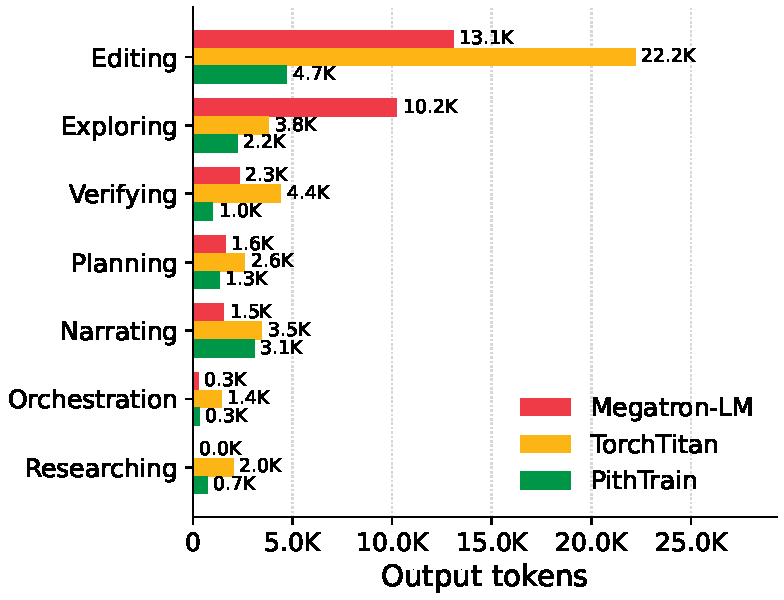
\includegraphics[width=\linewidth]{figures/token_breakdown.pdf}
    \caption{Per-category breakdown of output tokens.}
    \label{fig:moba-token-breakdown}
  \end{subfigure}
  \hfill
  \begin{subfigure}[t]{0.45\linewidth}
    \centering
    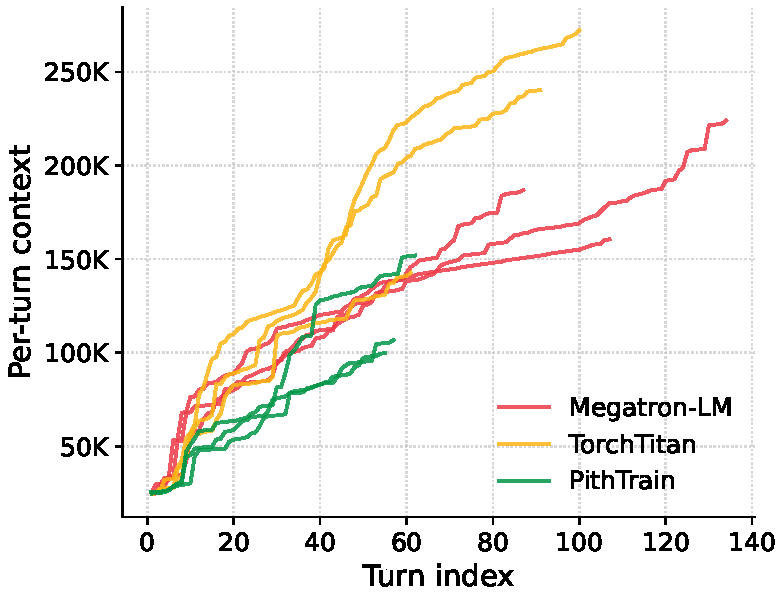
\includegraphics[width=\linewidth]{figures/context_trace.pdf}
    \caption{Per-turn context window over the session.}
    \label{fig:moba-context-trace}
  \end{subfigure}
  \caption{Agent behavior on integrating MoBA across frameworks.
  (\subref{fig:moba-token-breakdown}) reports the median output
  tokens per action category of three independent attempts;
  (\subref{fig:moba-context-trace}) shows the per-turn input-side
  context for each of three independent attempts.}
  \label{fig:moba-case-figures}
\end{figure}


To examine where per-framework differences in agent cost come from,
we conduct a case study on integrating MoBA, decomposing the
agent's output tokens by action
category\footnote{Thinking tokens are excluded as they are not
surfaced by the API.}~(\autoref{fig:moba-token-breakdown}) and
tracing its per-turn context
window~(\autoref{fig:moba-context-trace}). Editing dominates
across all three frameworks (\sys 4.7K, \megatron 13.1K,
\torchtitan 22.2K). \megatron also spends substantially more on
Exploring (10.2K vs.\ 3.8K for \torchtitan and 2.2K for \sys),
and its per-turn context sits well above \sys's. The agent reads
the codebase to locate edits and interpret tracebacks, so a
compact codebase with no implicit indirection lowers both
Exploring and per-turn context. \torchtitan's elevated Editing
and \textasciitilde2$\times$ context spike in two of three runs have a different
cause: the agent's initial implementation runs out of memory
(OOM), forcing repeated debug-edit cycles. This points to runtime
properties like memory headroom as a factor independent of
codebase structure.

Beyond \torchtitan's memory failures, we examine the other
failures the agent encountered. Across the three \sys runs, two
complete without any failure; the third hits a tensor-stride
mismatch in the agent's custom attention kernel, fixed in the same
file as the traceback. \megatron's three runs hit two distinct failures: two runs fail
with a duplicate command-line flag registration that conflicts with
one defined in framework code, and one run fails with a BF16
overflow in the agent's code. Each fix on \megatron spans multiple
files. This
contrast reflects \sys's compactness and absence of implicit
indirection, which keep each fix local to the agent's edit.




